\documentclass[border=10pt]{standalone}

\usepackage{tikz}
\usepackage{tikzsymbols}
\usetikzlibrary{calc,patterns,shapes.geometric}

\def\centerarc[#1](#2)(#3:#4:#5){\draw[#1] ($(#2)+({#5*cos(#3)},{#5*sin(#3)})$) arc (#3:#4:#5);}

\begin{document}
	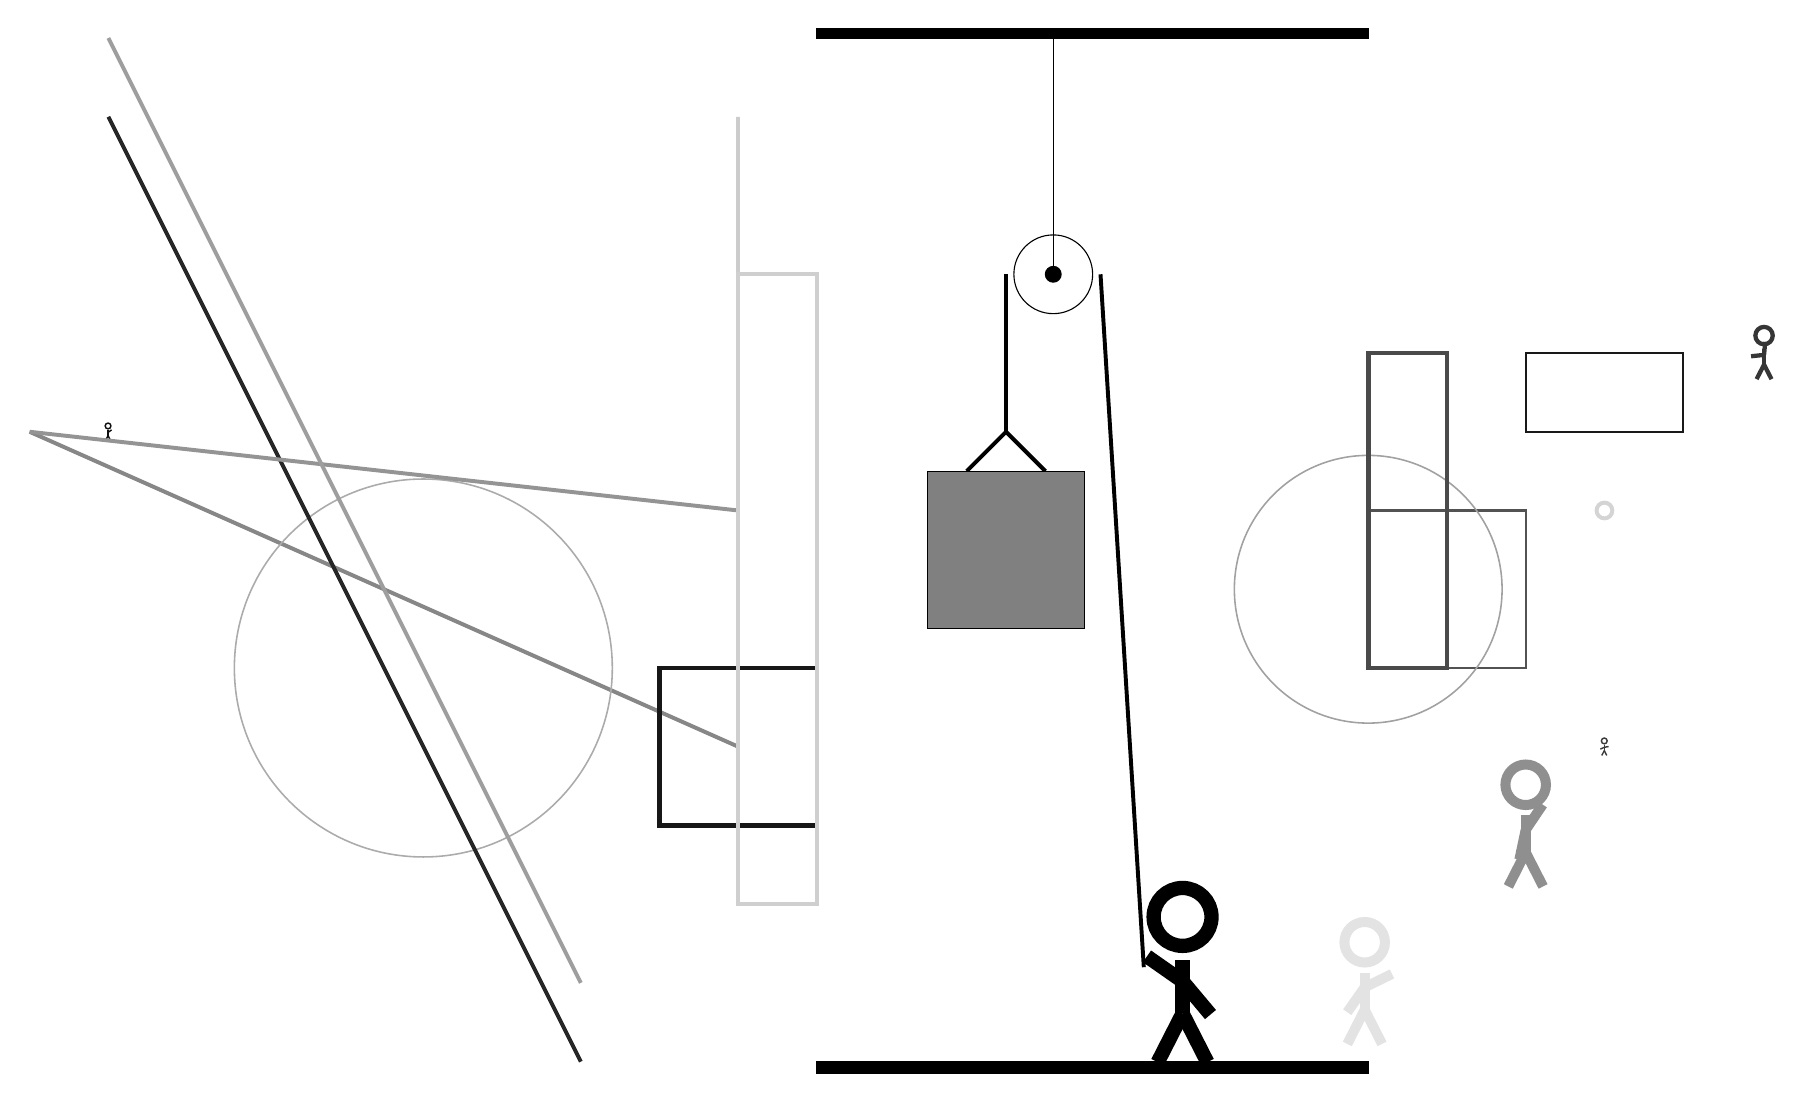
\begin{tikzpicture}
		%%%%% START %%%%%
		
		\draw[fill=black] (-2, 10) rectangle (5, 10.125);
		
		\draw (1, 7) circle (0.5);
		\draw[fill=black] (1, 7) circle (0.1);
		\draw (1, 10) -- (1, 7);
		
		\draw[line width=0.5mm] (-0.1, 4.5) -- (0.4, 5.0) -- (0.9, 4.5);
		\draw[fill=black!50] (-0.6, 4.5) rectangle (1.4, 2.5);
		
		\draw[line width=0.5mm] (0.4, 7) -- (0.4, 5.0);
		\centerarc[line width=0.5mm](1, 7)(0:180:0.6);
		\draw[line width=0.5mm](1.6, 7) -- (2.15, -1.8);
		
		\node[line width=0.6mm, color=black!11] at (5, -2) {\Strichmaxerl[7][55][26]};
		
		\node[line width=0.3mm, color=black!77] at (8, 1) {\Strichmaxerl[1][24][11]};
		\draw[line width=0.3mm, color=black!68] (5, 2) rectangle (7, 4);
		\draw[line width=0.5mm, color=black!47](-3, 1) -- (-12, 5);
		\draw [line width=0.2mm, color=black!33](-7, 2) circle (2.4);
		
		\draw[line width=0.5mm, color=black!20] (-3, 9) rectangle (-3, 7);
		\draw[line width=0.6mm, color=black!91] (-2, 2) rectangle (-4, 0);
		\node[line width=0.7mm, color=black!44] at (7, 0) {\Strichmaxerl[7][78][56]};
		\draw[line width=0.2mm, color=black!90] (7, 5) rectangle (9, 6);
		\draw[line width=0.5mm, color=black!85](-5, -3) -- (-11, 9);
		\draw [line width=0.2mm, color=black!37](5, 3) circle (1.7);
		\node[line width=0.4mm, color=black!94] at (-11, 5) {\Strichmaxerl[1][86][35]};
		\node[line width=0.6mm, color=black!79] at (10, 6) {\Strichmaxerl[3][6][85]};
		
		\draw[line width=0.5mm, color=black!42](-3, 4) -- (-12, 5);
		\draw[line width=0.5mm, color=black!38](-5, -2) -- (-11, 10);
		\draw [line width=0.5mm, color=black!17](8, 4) circle (0.1);
		
		\draw[line width=0.6mm, color=black!71] (6, 6) rectangle (5, 2);
		
		\draw[line width=0.5mm, color=black!13](-3, 7) -- (-2, 7);
		\draw[line width=0.5mm, color=black!19] (-3, 7) rectangle (-2, -1);
		
		\node at (2.6, -1.9) {\Strichmaxerl[10][-35][-50]};
		
		\draw[fill=black] (-2, -3) rectangle (5, -3.15);
		
		%%%%% END %%%%%
	\end{tikzpicture}
\end{document}